\subsection{Understanding Receiver Noise Figure: A Cheerful Dive into Clarity!}
\begin{tcolorbox}[colback=gray!10, colframe=black, title=E4C04]
What is the noise figure of a receiver?  
\begin{enumerate}[label=\Alph*.]
    \item The ratio of atmospheric noise to phase noise
    \item The ratio of the noise bandwidth in hertz to the theoretical bandwidth of a resistive network
    \item The ratio in dB of the noise generated in the receiver to atmospheric noise
    \item \textbf{The ratio in dB of the noise generated by the receiver to the theoretical minimum noise}
\end{enumerate} \end{tcolorbox}

\subsubsection{Concept Overview}
The noise figure (NF) is a critical parameter in receiver design and performance analysis in radio communications. It quantifies how much noise a receiver adds to the signal it processes, expressed in decibels (dB). Understanding the noise figure helps engineers evaluate the effectiveness of a receiver in different conditions, especially in weak signal environments.

\subsubsection{Additional Concepts Required}
To fully grasp the concept of noise figure, it is essential to understand the following:

1. \textbf{Signal-to-Noise Ratio (SNR):} This is the measure of the desired signal strength compared to the background noise level.
2. \textbf{Thermal Noise:} This is an unavoidable noise that is a result of the thermal agitation of electrons in conductive materials.
3. \textbf{Theoretical Minimum Noise:} This represents the lowest possible noise that can be generated by a resistor at a given temperature.

\subsubsection{Noise Figure Calculation}
The noise figure can be calculated using the formula:
\[
NF = 10 \log_{10} \left( \frac{N_{total}}{N_{theoretical}} \right)
\]
where:
- \(N_{total}\) is the total noise generated by the receiver,
- \(N_{theoretical}\) is the theoretical minimum noise.

In practical scenarios, if you know the total noise and the theoretical minimum noise your receiver operates under, you can plug those values into the formula above to compute the noise figure.

For instance, if a receiver generates a total noise of 10 nW and the theoretical minimum noise is 1 nW, the calculation would be:

\[
NF = 10 \log_{10} \left( \frac{10 nW}{1 nW} \right) = 10 \log_{10} (10) = 10 \text{ dB}
\]

\subsubsection{Diagram}
To provide a better understanding, we can visualize the relationship between signal, noise, and how the noise figure plays a role. Below is a simple representation using TikZ:

\begin{center}
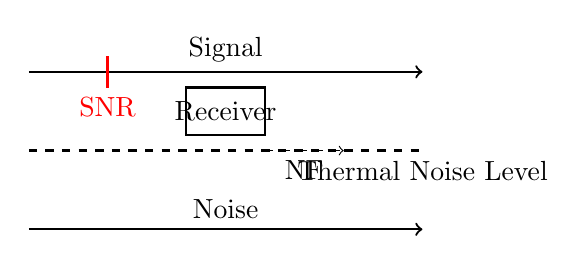
\begin{tikzpicture}
    % Signal Line
    \draw[->, thick] (0,0) -- (5,0) node[midway,above] {Signal};
    \draw[thick, red] (1,0.2) -- (1,-0.2) node[below] {SNR};

    % Noise Level
    \draw[->, thick] (0,-2) -- (5,-2) node[midway,above] {Noise};
    \draw[thick, dashed] (0,-1) -- (5,-1) node[below] {Thermal Noise Level};

    % Receiver Box
    \draw[thick] (2,-0.8) rectangle (3,-0.2);
    \node at (2.5,-0.5) {Receiver};
    
    % Noise Figure Annotation
    \draw[dashed,->] (3,-1) -- (4,-1) node[midway,below] {NF};
\end{tikzpicture}
\end{center}

This diagram illustrates the basic concept of how noise and signal interact within a receiver and highlights where the noise figure comes into play.